

\chapter{PHILLIPO}

PHILLIPO é um \emph{solver} para análise de em estruturas discretizadas por elementos finitos, com algumas otimizações computacionais relacionadas a paralelismo e matrizes esparsas, e que visa constituir-se como exemplo didático na implementação legível e concisa dos algoritmos de elementos finitos em Julia no âmbito acadêmico do campus CCT, da UDESC. PHILLIPO é um programa de código aberto, que é distribuído em um repositório público\footnotemark[1]{} sob a licença LGPL\footnotemark[2]{}. Portanto, sua utilização é gratuita e livre para fins acadêmicos e comerciais, que incluem a modificação, implementação e venda de qualquer parte do programa, como também da documentação que o acompanha; só se resguarda, entretanto, a devida citação deste documento. A logo de PHILLIPO é mostrada na figura \ref{fig:log_phillipo}.
\footnotetext[1]{O repositório é mantido no GitHub, assim como o presente documento em formato Latex: \url{https://github.com/lucas-bublitz/PHILLIPO}}
\footnotetext[2]{O GiD, interface de pré e pós-processamento, é um software distribuído comercialmente, e não está sujeito à mesma licença que PHILLIPO.}

\begin{figure}[hbtp]
    \centering
    \caption{Logo estilizada de PHILLIPO.jl}
    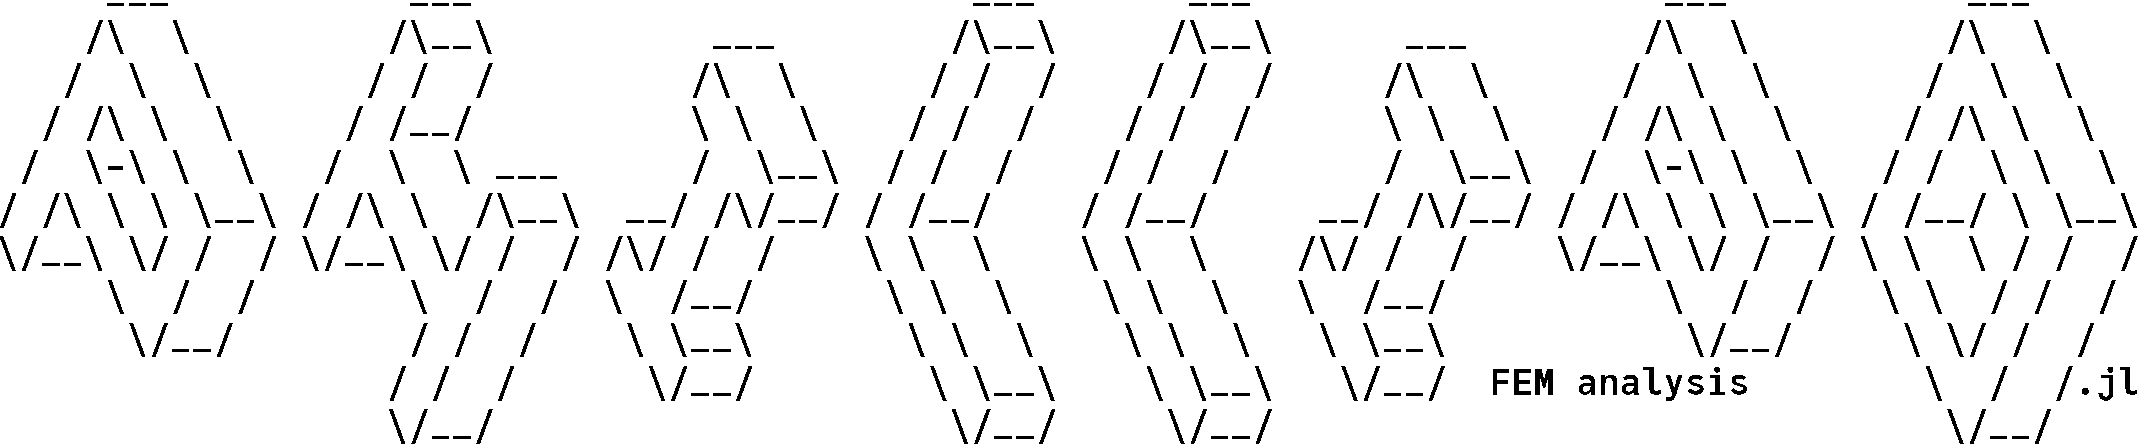
\includegraphics[width = \textwidth]{Figuras/logo_phillipo.pdf}
    \label{fig:log_phillipo}
\end{figure}

Um \emph{solver}, ou em melhor português, um solucionador em MEF não é uma novidade no mundo acadêmico, nem no comercial. Softwares como Calculix (que é distribuído integrado com o FreeCAD) e o FreeFEM, que já conta com 7 mil commits em seu repositório, são continuamente produzidos e aprimorados desde antes da virada do milênio, um trabalho que demanda tempo e uma comunidade bem ativa. Deste modo, a pretensão de PHILLIPO não é fornecer uma alternativa a esses softwares, muito menos servir de módulo ou biblioteca para agregar algum deles, além do mais, a elaboração de programas robustos e confiáveis é um trabalho demorado e de muitas pessoas.

A pretensão de PHILLIPO é construir uma aplicação simples utilizando o MEF, que possa aproveitar algumas ferramentas de construção de código em Julia, como paralelismo e despachos múltiplos, para apresentar mais uma referência de programação em engenharia no campus CCT, da UDESC, e, deste modo, evidenciar que é possível construir aplicações do MEF de forma simples e legível, e por meio de uma linguagem de programação moderna, como Julia.

Neste capítulo é apresentado como é feita a distribuição, instalação e como se dá o funcionamento de PHILLIPO, dividido em duas partes. A primeira, descrevendo o fluxo de execução normal do programa, isto é, utilizando o GID como interface de pré e pós-processamento, e, a segunda, esmiuçando o código, tanto do módulo PHILLIPO, quanto dos arquivos de integração com o GID.

\section{Distribuição pelo Pkg.jl e importação dos \emph{Problems types} no GID}

O Pkg.jl é o gerenciador de pacotes anexado à Julia, tal como PIP é anexado ao Pyhton. Ele é responsável por distribuir, gerir e empacotar os módulos da linguagem, permitindo relacionar dependências e controlar versionamento. PHILLIPO é distribuído por meio do Pkg.jl, porém, não pelo repositório oficial\footnote{Há uma série de critérios para que um módulo seja adicionado ao repositório oficial do Pkg.jl, além disso, não é objetivo de PHILLIPO ser distribuido massivamente.}, mas pelo próprio repositório deste trabalho, que pode ser utilizado para o mesmo fim, pela função \emph{add}. A utilização do \emph{Pkg.jl} determinou a estrutura de a estrutura dos arquivos de código-fonte de PHILLIPO, conforme o próprio manual do pacote\footnote{Acessível em \url{https://pkgdocs.julialang.org/v1/}}.

Como PHILLIPO foi encapsulado em um módulo, pode ser facilmente distribuído iniciando uma sessão Julia e executando:
\begin{lstlisting}
    add https://github.com/lucas-bublitz/PHILLIPO.jl
\end{lstlisting}

O Pkg.jl então trata de buscar as dependências do módulo, isto é, os módulos que são importados para uso interno de PHILLIPO: o \emph{SparseArrays}, que fornece as estruturas e funções para alocar e manipular eficientemente matrizes esparsas, o \emph{LinearAlgebra}, implementação do LAPACK em Julia, e o \emph{JSON}, um parser de objetos em JSON para dicionários. No arquivo \emph{Projecy.toml} é possível encontrar tanto essa lista de dependência, e no \emph{Manifest.toml}, são listadas as dependências das dependências, isto é, quais módulos cada módulo importado por PHILLIPO importa para si. \footnote{O versionamento é importante pois permite que a compilação do pacote seja feita utilizando exatamente os códigos dos módulos de quando foi desenvolvido, assim baixando o risco de resultados inesperados devido a uma alteração no funcionamento de um módulo exterior ao que se trabalha. }

PHILLIPO utiliza a interface GID para gerar as malhas e definir as condições de contorno. A integração desses programas é feita pelo conjunto de arquivos presente presentes na pasta \emph{\textbackslash GID connections}: \emph{PHILLIPO.gid} e \emph{PHILLIPO3D.gid}, que são os \emph{Problem types} do GID para PHILLIPO, e \emph{link.jl}, que é o arquivo que é chamado pelo \emph{script} de execução do GID, e que importa o módulo PHILLIPO.jl e o executa. O conteúdo dessa pasta deve ser copiado para a pasta \emph{\dots\textbackslash GiD 16.1.6d \textbackslash ProblemTypes}, localizada onde o próprio GID está instalado\footnote{O caminho para a pasta \emph{ProblemTypes} pode variar de acordo com a versão do GID, e com o sistema operacional.}, para que sejam automaticamente carregados durante a inicialização do GID\footnote{Também é possível importar \emph{Problem types} dentro da interface do GID, entretanto, desse modo, a importação não é permanente.}.

\section{Fluxo de execução}

O fluxo de execução é uma ferramenta de projeto que tem como objetivo descrever a ordem e as condições que determinadas seções do código são executadas. A utilização de PHILLIPO.jl segue os digramas das figuras \ref{fig:fluxograma_GID} e \ref{fig:fluxograma_PHILLIPO}. Esses diagramas não representações simplificados e parciais, e não utilizam um padrão ou simbologia formal que é própria desses diagramas.
\begin{figure}[hbtp]
    \centering
    \caption{Fluxograma de execução: GID}
    \includegraphics[width = \textwidth]{Figuras/fluxograma_GID.pdf}
    \label{fig:fluxograma_GID}
\end{figure}

\begin{figure}[hbtp]
    \centering
    \caption{Fluxograma de execução: PHILLIPO.jl}
    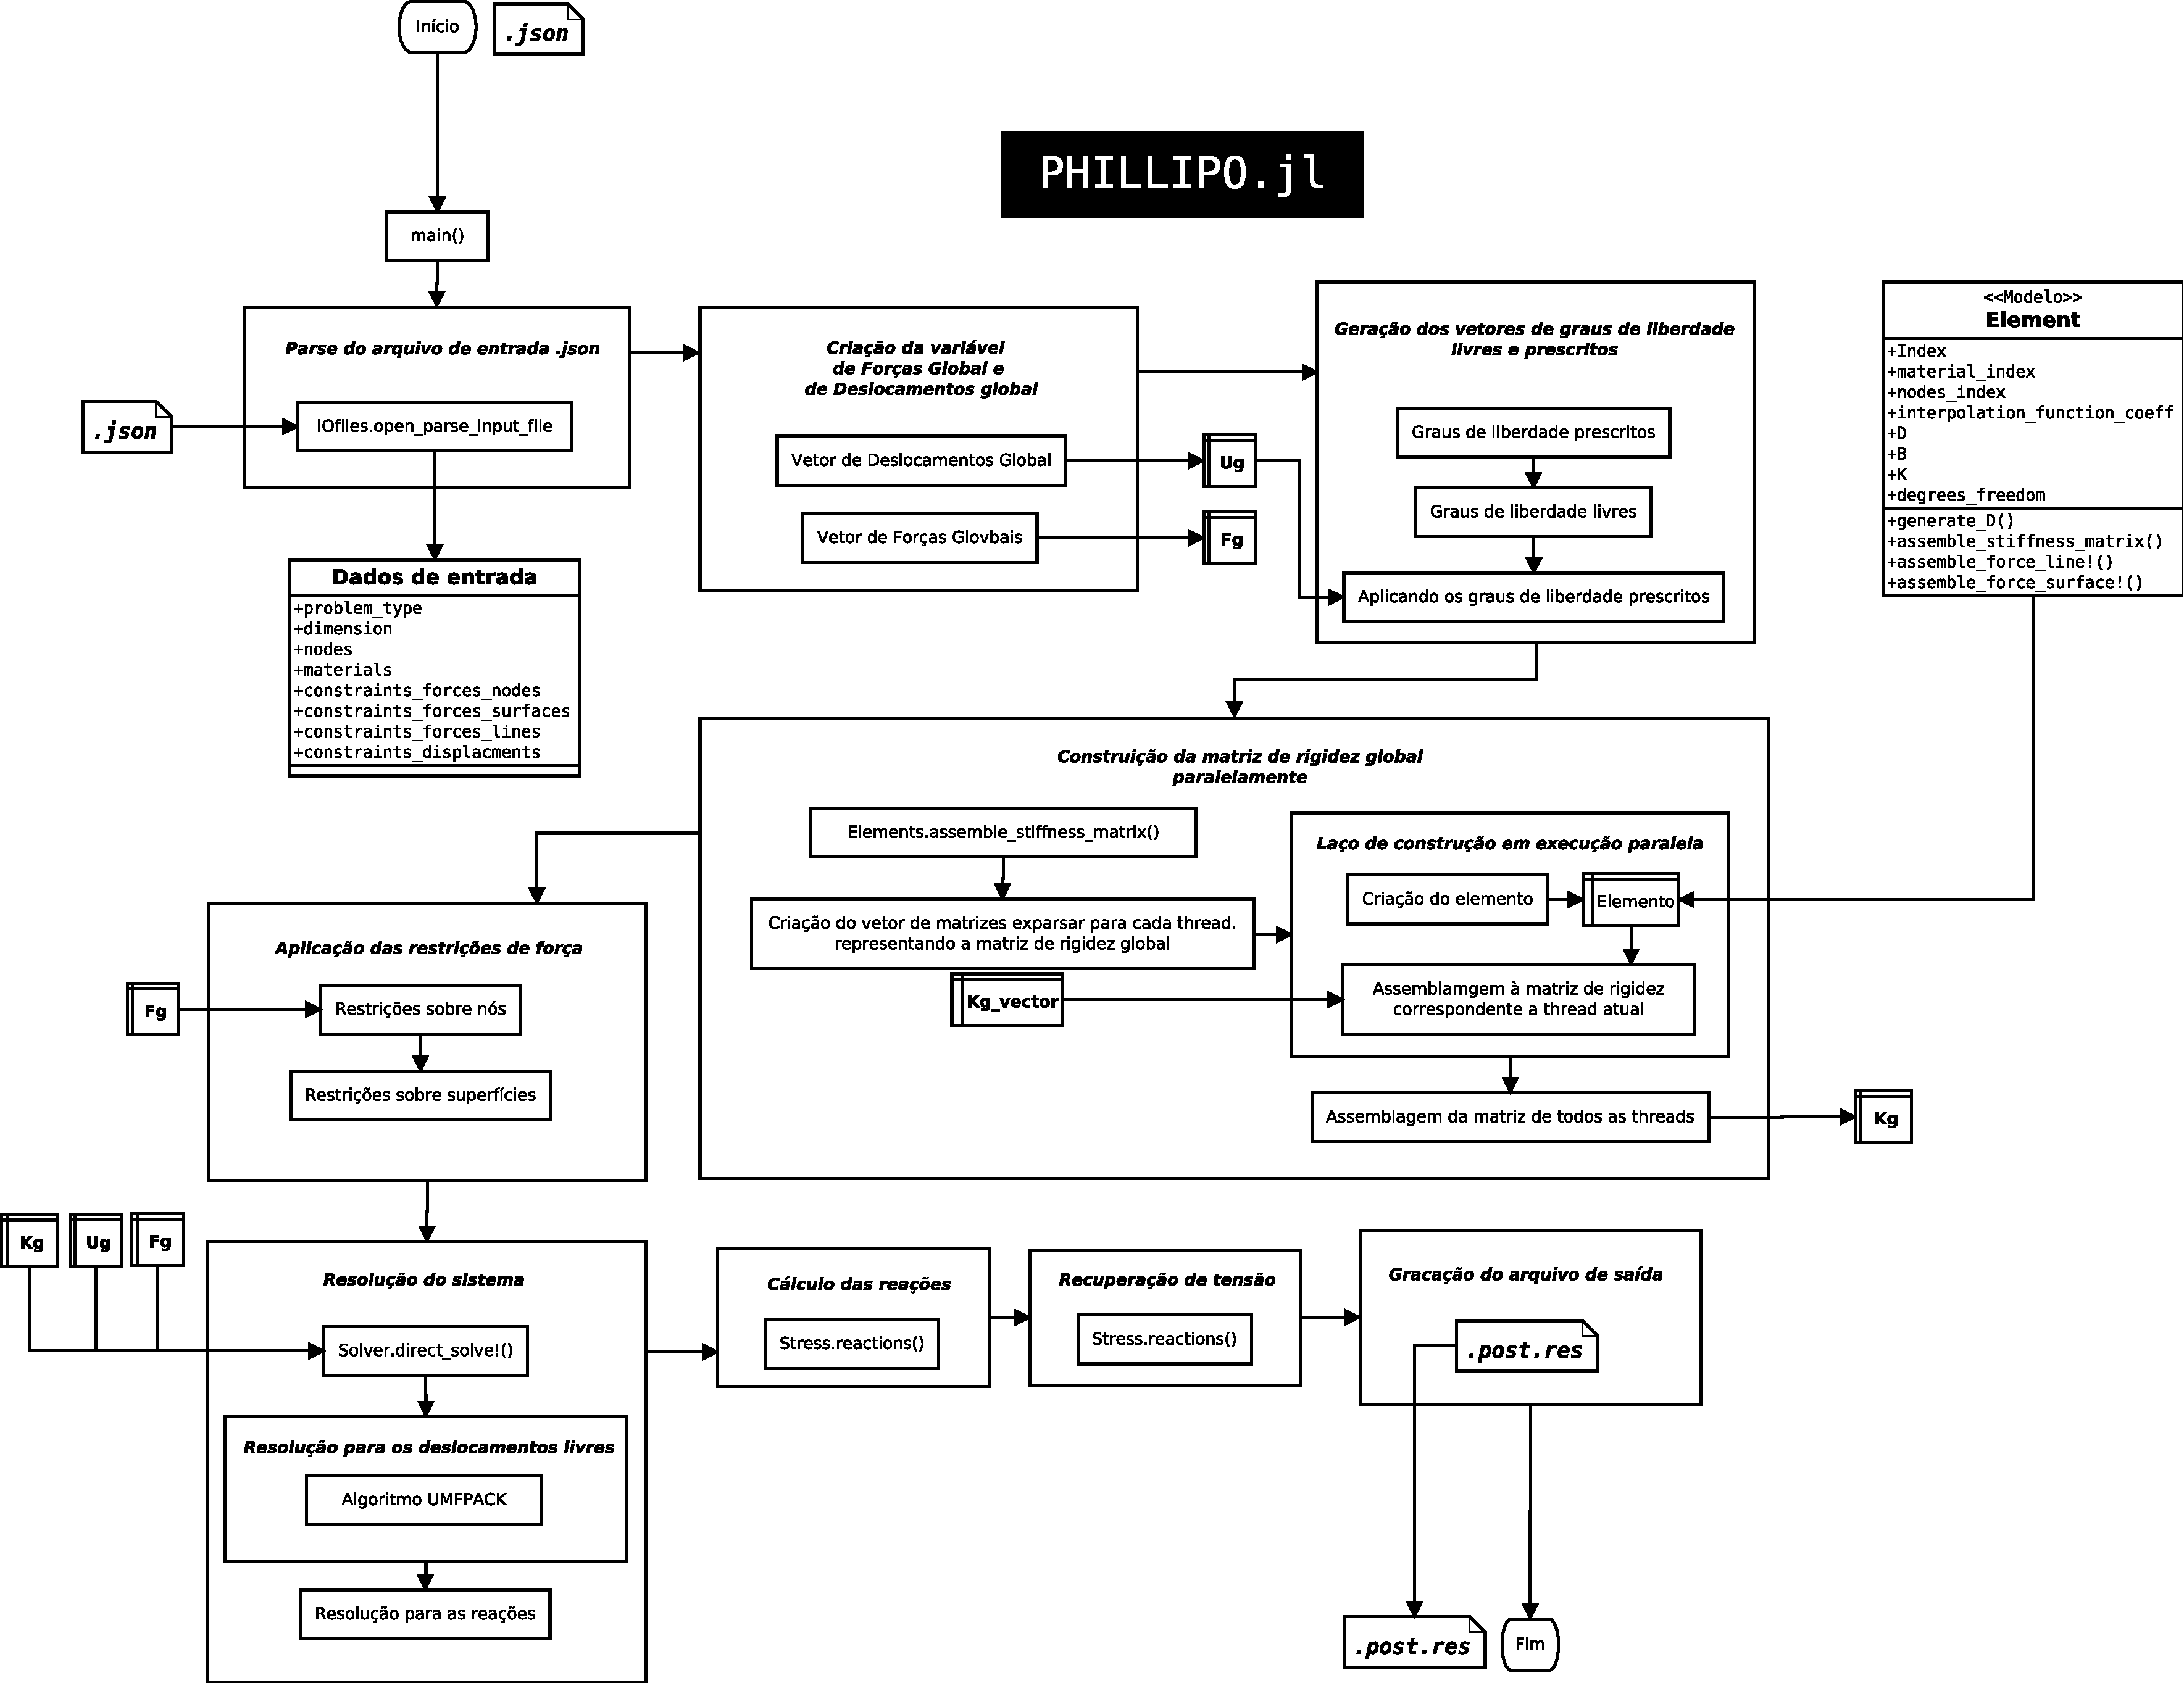
\includegraphics[width = \textwidth]{Figuras/fluxograma_PHILLIPO.pdf}
    \label{fig:fluxograma_PHILLIPO}
\end{figure}

Nesses diagramas, é possível separar a execução de uma utilização normal do software em três partes principais:

\begin{enumerate}
    \item Pré-processamento;
        Parte em que ocorre a criação da geometria, a definição das propriedades dos materiais, das condições de contorno e das cargas aplicadas, assim como a geração da malha e elementos.
    \item Processamento;
        Parte em que é chamada uma sessão Julia para carregar o módulo PHILLIPO.jl, que é responsável por ler os arquivos de entrada, e executar o algoritmo de elementos finitos, gerando os arquivos de saída para o GID.
    \item Pós-processamento;
        Parte em que o GID lê os arquivos de saída, e gera os gráficos de resultados.
\end{enumerate}

\subsection{Pré-processamento}

O pré-processamento é realizado totalmente pelo GID (figura \ref{fig:fluxograma_GID}), e consisti na definição da geometria, das condições de contorno, do material e na geração de malha, e segue:

\begin{enumerate}
    \item Definição do \emph{Problem type}. Caso o problema físico seja modelado em duas dimensões, deve-se escolher o \emph{Problem type} \emph{PHILLIPO}, caso seja modelado em três dimensões, deve-se escolher o \emph{Problem type} \emph{PHILLIPO3D}. Essa escolha define quais arquivos serão utilizados para a definição das condições de contorno, dos materiais, e como será a geração da malha. O GID cria então uma pasta onde os arquivos do problema serão salvos.

    \item \textbf{Definição da geometria do problema,} que pode ser tanto construída utilizando as ferramente CAE do próprio GID, como também, importada de um arquivo externo de algum outro software CAD cujo formato seja reconhecido pelo GID \footnote{O GID reconhece uma grande variedade de arquivo de entrada (sejam de geometria, malhas, condições de contorno), inclusive arquivos próprios de programas comerciais, como ANSYS e Abaqus;}.

    \item \textbf{Definição das características do material,} como também as condições de contorno: sejam elas deslocamentos sobre pontos, linhas e superfícies, ou carregamentos concentrados sobre pontos, ou carregamentos distribuídos sobre linhas e superfícies. \footnote{Carregamentos sobre linha só estão disponíveis para o \emph{Problem type} \emph{PHILLIPO}.}

    \item \textbf{Geração da malha,} que pode ser amplamente configuras pelas ferramentas oferecidas pelo GID para gerar malhas estruturadas ou não estruturas, com refinamentos em determinadas regiões, e com a possibilidade de se definir o tipo de elemento a ser utilizado. 
    \item \textbf{Chamamento da função de CALCULAR.}
\end{enumerate}

A função de CALCULAR do GID, executa o arquivo \emph{.bat} do \emph{problem type}: deleta possíveis arquivos de saída anteriores, e gera os arquivos de saída \emph{.dat}\footnote{Embora o arquivo esteja nomeado no formato \emph{dat} ele, na verdade, é um \emph{.json}, pois esse é o padrão de entrada para PHILLIPO.}, assim como os arquivos de \emph{log}, e cria a sessão Julia, chamando para ser executado nela o arquivo \emph{link.jl}. 

Na sessão Julia, o módulo PHILLIPO.jl é importado, momento em que ocorre a pré-compilação do código, e, em seguida, o chamamento da função principal do módulo \emph{PHILLIPO.main}, passando como parâmetros os caminhos para o arquivo \emph{.json} e o caminho de saída do resultado da análise, assim iniciando o processamento.

\subsection{Processamento}

O processamento é realizado dentro da sessão Julia, executando a função principal de \emph{PHILLIPO.main} (figura \ref{fig:fluxograma_PHILLIPO}), e consiste nas seguintes etapas:
\begin{enumerate}
    \item \textbf{Leitura do arquivo de entrada.} O arquivo \emph{.json} é lido e convertido em um dicionário pelo \emph{parser} JSON, cujos dados são distribuídos nas variáveis do problema.
    \item \textbf{Definição dos graus de liberdade livres e prescritos.} Conforme sãos as restrições de deslocamento, o programa calcula a numeração dos graus de liberdade prescritos, e os armazena em um vetor.
    \item \textbf{Construção da matriz global de rigidez paralelamente.} Nessa etapa, o programa chama as funções de construção de elemento paralelamente, utilizando uma macro do módulo \emph{Threads}, para construir a matriz global de rigidez, que é salva no formato COO (um formato de matriz esparsa que armazena os valores em um vetor único cuja ordem não importa para a interpretação da matriz, o que facilita a execução paralela). Após a construção da matriz global de rigidez, é feita a conversão para o formato CSR. 
    \item \textbf{Aplicação das restrições de forças.} As restrições de forças são aplicadas sobre o vetor de forças prescritas. Dependendo do tipo (sobre linhas ou superfícies), são calculadas as forças nodais equivalentes.
    \item \textbf{Resolução do sistema.} Com a matriz global de rigidez e o vetores de deslocamentos e forças nodais, o programa decompõe o sistema pelos graus de liberdade livres e prescritos, e o resolve diretamente, utilizando o método mais apropriado, determinado pelo módulo \emph{LinearAlgebra}, levando em consideração as características da matriz de rigidez global.
    \item \textbf{Cálculo das reações e recuperação de tensão.} O programa calcula as reações de apoio, utilizando os graus de liberdade prescritos, e, em seguida, calcula as tensões, chamando, novamente, as funções de construção de elementos para resgatar as matrizes de rigidez locais.
    \item \textbf{Geração do arquivo de saída.} O programa gera o arquivo de saída, no formato \emph{.dat}, que é lido pelo GID para gerar os gráficos de resultados.

\end{enumerate}

Com o fim da execução da função principal, é encerrada a sessão Julia e, e é chamado o programa Notepad para a abrir o arquivo \emph{.log}, onde algumas informações de debug foram impressas durante o processamento. 

\section{Integração com GID}

O GID é um software utilizado como pré e pós-processamento. Com ele é possível criar a geometria do problema, definir as propriedades dos materiais, as condições de contorno, as cargas aplicadas, e, principalmente, gerar a malha de elementos. Além de se ser possível a integração com um \emph{solver} qualquer, por meio de um conjunto de arquivos de entrada e saída (ambos configurados de forma a permitir uma certa flexibilidade nessa integração), cuja execução é controlada por um \emph{script} em Batch, o que possibilita a automatização do processo de simulação. Nesta seção é abordado como é feita e integração entre o GID e PHILLIPO, por meio das pastas \emph{PHILLIPO.gid} e \emph{PHILLIPO3D.gid}, sendo que, como a nomeação dos arquivos sugere, a primeira é utilizada para problemas bidimensionais, e a segunda para problemas tridimensionais.

\subsection{PHILLIPO.gid}

O GID pode ser configurado para operar como pré e pós-processamentos de diversos programas, como o Abaqus, o Ansys, o Calculix..., por meio de um \emph{Problem type}, que é como o GID chama o conjunto de arquivos que configuram o formato de saída dos dados, a criação de determinadas propriedades para as condições de contorno e materiais, como também automatizar a execução da simulação, chamando o programa. Pode-se dizer que o \emph{Problem type} é uma interface para que as informações contidas nos arquivos gerados pelo GID (geometria, malha, condições de contorno etc.) sejam salvas em um formato que o programa, o \emph{solver}, possa interpretar, ao passo que o \emph{script} de execução automatiza o chamamento desse, e a simulação seja iniciada. 

Na pasta \emph{PHILLIPO.gid} é possível encontrar os seguinte arquivos:

\begin{enumerate}
    \item \emph{PHILLIPO.cnd}: define as condições de contorno e como são aplicadas;
    \item \emph{PHILLIPO.prb}: define as entradas de informações gerais;
    \item \emph{PHILLIPO.mat}: define as características dos materiais utilizados para os elementos;
    \item \emph{PHILLIPO.bas}: configura o arquivo de saída do GID para ser interpretado por PHILLIPO.jl;
    \item \emph{PHILLIPO.bat}: \emph{script} para chamar uma sessão Julia, chamando \emph{link.jl};
    \item \emph{link.jl}: importa o módulo PHILLIPO e o executa.
\end{enumerate}

O primeiro arquivo do \emph{Problem type} de PHILLIPO é \emph{PHILLIPO.cnd}, que define as condições de contorno e sobre quais entidades, leia-se nós, elementos ou geometrias (superfícies, volumes, linhas etc.), são aplicadas, por meio de uma sintaxe específica \footnote{No manual do usuário do GID, acessível em \url{https://gidsimulation.atlassian.net/wiki/spaces/GUM/overview}, é possível encontrar a descrição o funcionamento de toda essa sintaxe, que compreende desde esse arquivo de condições de contorno, como também, dos outros que compões a construção do \emph{problem type}.}, uma forma de marcação de texto, que é interpretada pelo GID.

\begin{figure}[hbtp]
    \caption{Parte do arquivo de condições de contorno: PHILLIPO.cnd}
    \lstinputlisting[lastline=10]{../GID connection/PHILLIPO.gid/PHILLIPO.cnd}
    \label{fig:PHILLIPO.cnd}
\end{figure}

Em sua representação parcial, da figura \ref{fig:PHILLIPO.cnd}, é possível notar a construção de uma condição de contorno por meio de um bloco que inicia na linha 1, com a expressão \emph{CONDITION: Constraint\_displacement\_point}, que também nomeia esta condição, referente a restrição de deslocamento em pontos (entidade geométrica discretizada por um nó), e que acaba com \emph{END CONDITION}. Dentre essas linhas, são definidas as formas e os valores que essa condição vai aplicar sobre a geometria selecionada, neste caso, os pontos. Na linha 2, é definido, justamente, sobre qual entidade geométrica se aplica essa condição: pontos. Na próxima linha, é definido como que essa informação, que foi associada à entidade geométrica se traduz na malha: essa condição é aplicada sobre os nós que cujo ponto foi discretizado. \footnote{Isso se deve porque a malha é criada sobre a geometria, posteriormente à aplicação das condições de contorno sobre aquela.} As linhas seguintes, 4 a 9, se referem aos valores da condição, neste caso, aos deslocamentos prescritos sobre os nós nas direções de \emph{X}, \emph{Y} e \emph{Z}. 

Na condição \emph{Constraint\_force\_line} (figura \ref{fig:PHILLIPO.cnd_2}), o processo é análogo. A restrição de carregamento uniforme é aplicada sobre uma linha (o tipo de geometria), e, diferentemente da anterior, é traduzida sobre as faces. Nesse caso bidimensional, é o segmento de reta determinado pelos nós nas extremidades. Os campos \emph{X}, \emph{Y} e \emph{Z}, referem-se ao vetor dessa carregamento uniformeS.

\begin{figure}[hbtp]
    \caption{Parte do arquivo de condições de contorno: PHILLIPO.cnd}
    \lstinputlisting[firstline=36,lastline=45]{../GID connection/PHILLIPO.gid/PHILLIPO.cnd}
    \label{fig:PHILLIPO.cnd_2}
\end{figure}

O arquivo \emph{PHILLIPO.prb} (figura \ref{fig:PHILLIPO.prb}) define as entrada de informações gerais ao problema, ou seja, que não são aplicados diretamente sobre a geometria. Somente um campo foi utilizado e se refere ao tipo do estado plano (EPD ou EPT). A sintaxe da linha 3 é indica que esse campo só possa ser preenchido por essas duas opções, no formato \emph{drop-down list}.
\begin{figure}[hbtp]
    \caption{Arquivo de dados gerais: PHILLIPO.prb}
    \lstinputlisting[firstline=1,lastline=8]{../GID connection/PHILLIPO.gid/PHILLIPO.prb}
    \label{fig:PHILLIPO.prb}
\end{figure}

O arquivo \emph{PHILLIPO.mat} (figura \ref{fig:PHILLIPO.mat}) define as características dos materiais implementados. Somente um material foi definido, o aço AISI 4340, com os campos de módulo de elasticidade, coeficiente de Poisson e massa específica.

\begin{figure}[hbtp]
    \caption{Arquivo de materiais: PHILLIPO.mat}
    \lstinputlisting[firstline=1,lastline=8]{../GID connection/PHILLIPO.gid/PHILLIPO.mat}
    \label{fig:PHILLIPO.mat}
\end{figure}

O arquivo \emph{PHILLIPO.bas} configura o arquivo de saída do GID. Esse arquivo intercala o conteúdo explicito do arquivo de saída (as partes invariáveis), com trechos de programação, responsáveis por imprimir os valores dinâmicos, aqueles referentes ao problema em si, como as coordenadas dos nós, a conectividade dos elementos etc.\footnote{Esse modo de compor os arquivo, misturando textos estáticos e programação é similar aos arquivos em PHP. Isso numa utilização mais clássica.} A separação entre texto e programa se dá pelo caractere \emph{*} no início da linha, indicando que toda ela é uma instrução para ser executada. 

O arquivo gerado é do formato \emph{.json}, o que pode ser não usual para aplicações do MEF. Entretanto, esse formato é amplamente utilizado para troca de dados entre aplicações, e, por isso, pode ser facilmente lido por um módulo já consolidado em Julia, o \emph{JSON.jl}\footnote{JSON se refere a \emph{JavaScript Object Notation}, um formato de texto para representar objetos na linguagem JavaScript, que se tornou padrão na implementação de APIs.}. 

Para gerar as listas de elementos triangules, foi escrito o seguinte código, dentro do arquivo emph{PHILLIPO.bas}:
\lstinputlisting[firstline=10,lastline=16]{../GID connection/PHILLIPO.gid/PHILLIPO.bas}

Na linha 1 é definido o nome do campo \emph{"nodes"}, separado pelo características \emph{:} inicia a declaração do valor daquele campo: uma lista \emph{[}\footnote{Essa sintaxe de listas e \emph{literals} é próprio do JavaScript.}. Na linha 2, é iniciado um laço de repetição, que percorre todos os nós, e, para cada um, é adicionado um elemento à lista, que é composto por um par de coordenadas, separadas por vírgula, e envolvidas por colchetes, pois cada nó é presentando por um vetor que contem suas coordenadas. Na linha 5, é fechado o laço de repetição, e, na linha 6, é fechado o campo \emph{]}. 

Esse padrão se repete para o elementos também, com a diferença que estes, dependendo do seu tipo (CST ou tetraedro), são listas dentro da tupla que representa dos os elementos. Na figura \ref{fig:PHILLIPO.bas}, é possível nota essa hierarquia dos dados na estrutura de entrada de PHILLIPO.

No exemplo da figura

\begin{figure}[hbtp]
    \caption{Arquivo de saída do quarto caso de verificação: 4 verification case.dat}
    \lstinputlisting{../verification/4 verification case/4 verification case.gid/4 verification case.dat}
    \label{fig:PHILLIPO.bas}
\end{figure}

O arquivo \emph{PHILLIPO.bat} (figura \ref{fig:PHILLIPO.bat}) é um \emph{script} que é chamado pela função CALCULAR do GID, para iniciar a análise do problema. É um arquivo de linhas de comando (ou arquivo de lote)\footnote{Comandos utilizados dentro do terminal do sistema: o CMD.} para o sistema operacional Windows\footnote{Por conta disso, o \emph{PHILLIPO.gid} só funciona em sistemas Windows.}.

Nas linhas 1 a 3, são feitas as exclusões de possíveis arquivos restantes de análises passadas. Na linha 4, é chamada a sessão Julia, passando como parâmetro o arquivo \emph{link.jl}, o caminho absoluto do arquivo de entrada \emph{.dat} e o local em que o arquivo de saída deve ser gravado. No final da linha, os operadores right-shift \emph{>>} redirecionam o debug da execução de PHILLIPO para o arquivos \emph{.log} e \emph{.error.log}. Na linha 5, o arquivo log de erro é aglutinado ao arquivo de log para que, quando a linha 5 for executada, o aplicativo Notepad exiba os dois conteúdos juntos\footnote{Assim foi implementado porque se o mesmo arquivo receber o fluxo de texto, o conteúdo dos erros sobrescrevem aos normais}. 

A flag \emph{-t} com o parâmetro \emph{auto} na linha 4, indica que a sessão Julia deve ser iniciado utilizado um número de threads disponibilizados pelo sistema \footnote{O parâmetro pode ser alterado para forçar a sessão Júlia a usar mais threads.}. Isso é importante para que ocorra a montagem da matriz global de rigidez paralelamente.

\begin{figure}[hbtp]
    \caption{Arquivo de execução: PHILLIPO.bat}
    \lstinputlisting{../GID connection/PHILLIPO.gid/PHILLIPO.bat}
    \label{fig:PHILLIPO.bat}
\end{figure}

O arquivo \emph{link.jl} (figura \ref{fig:link.jl}) é o arquivo que executado dentro da sessão Julia. Ele recebe esse nome porque é o arquivo que faz a ligação entre a execução do GID e o módulo PHILLIPO.jl, e, por não estar previsto dentro da estrutura de um \emph{problem type}, recebe um nome diferenciado. Nele é apenas importado o módulo PHILLIPO.jl  (linha 1) e chamado a função principal do módulo (linha 2), passando como parâmetros o caminho para o arquivo de entrada e o caminho para a gravação do arquivo de saída \footnote{ARGS é um vetor presente em toda a sessão Julia, que recebe os parâmetros passados para o executável que a iniciou.}. A última linha é responsável por garantir o encerramento da sessão Julia.

A macro \emph{@time} é responsável por fornecer algumas informações sobre o tempo de execuções do módulo (como também memória alocada e tempo dedicado à compilação ao \emph{Garbage Collector}). É uma ferramenta de debug, e seu retorno é impresso no arquivo \emph{.log}.

\begin{figure}[hbtp]
    \caption{Arquivo de execução: link.jl}
    \lstinputlisting{../GID connection/PHILLIPO.gid/link.jl}
    \label{fig:link.jl}
\end{figure}

\section{Estrutura do módulo PHILLIPO.jl}

O código-fonte de PHILLIPO foi organizado em seis módulos, ao longo de sete arquivos \emph{.jl}, agrupando as funções em categorias conforme sua aplicação. O início da definição do módulo de PHILLIPO é o arquivo homônimo, localizado na raiz da pasta \emph{src} do repositório.
